\documentclass[10pt,a4paper,final]{article}
\usepackage[latin1]{inputenc}
\usepackage{amsmath}
\usepackage{amsfonts}
\usepackage{amssymb}
\usepackage{graphicx}
\setlength{\topmargin}{-.5in}
\setlength{\textheight}{9in}
\setlength{\oddsidemargin}{.125in}
\setlength{\textwidth}{6.25in}
\author{Dennis Ideler}
\title{MATH 2P71: Intro to Combinatorics\\Assignment 1: Counting}
\begin{document}
\maketitle

\begin{enumerate}
\item % Q1
(a) Let $A = \{a, b, c, d, e\}$.
List all subsets of A containing $\{a, e\}$ but not containing $c$.\\
\\
We can use binary representation of the set to find all subsets that satisfy the requirements.
The cardinality of $A$ is $|A|$ = 5. The number of subsets of $A$ is $2^{|A|} = 2^5 = 32$.
We can use 5 bits to represent all subsets.
We know that the subsets must contain $\{a,e\}$ and cannot contain $c$,
so the bits for $a$ and $e$ will always be set and the bit for $c$ will never be set.\\
\begin{tabular}{c c c}
$10001$ & $\Rightarrow$ & $\{a,e\}$\\
$10011$ & $\Rightarrow$ & $\{a,d,e\}$\\
$11001$ & $\Rightarrow$ & $\{a,b,e\}$\\
$11011$ & $\Rightarrow$ & $\{a,b,d,e\}$\\
\end{tabular}

Another method is to break down the selection of subsets into independent decisions.
This is visualized in figure~\ref{decisiontree}.\\
\begin{figure}[h!]
  \centering
    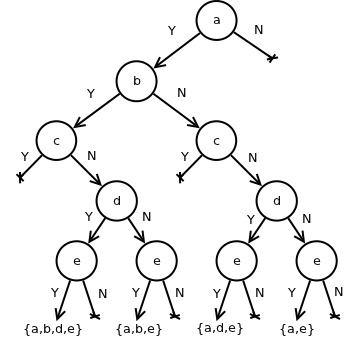
\includegraphics[scale=0.5]{1ab.png}
  \caption{A pruned decision tree for selecting subsets.}
  \label{decisiontree}
\end{figure}

(b) Let $B = \{c, d, e\}$. List all subsets of $A$ whose intersection with $B$ has 1 element,
i.e. $|A \cap B| = 1$.\\
\\
An easy way to answer this is by representing the subsets of $A$ in binary.\\
For bits $a$ and $b$, we have $2^2 = 4$ options (either bit can be set or unset,
it makes no difference on the outcome).
For bits $c$, $d$, and $e$, only one \emph{must} be set at any given time, thus 3 options.
There are then $4 \times 3 = 12$ subsets of $A$ that qualify:
\begin{tabular}{c c c}
$ab\,cde$ & & subsets\\
$00\,001$ & $\Rightarrow$ & $\{e\}$\\
$00\,010$ & $\Rightarrow$ & $\{d\}$\\
$00\,100$ & $\Rightarrow$ & $\{c\}$\\
\\ % or \hline
$01\,001$ & $\Rightarrow$ & $\{b,e\}$\\
$01\,010$ & $\Rightarrow$ & $\{b,d\}$\\
$01\,100$ & $\Rightarrow$ & $\{b,c\}$\\
\\ % or \hline
$10\,001$ & $\Rightarrow$ & $\{a,e\}$\\
$10\,010$ & $\Rightarrow$ & $\{a,d\}$\\
$10\,100$ & $\Rightarrow$ & $\{a,c\}$\\
\\ % or \hline
$11\,001$ & $\Rightarrow$ & $\{a,b,e\}$\\
$11\,010$ & $\Rightarrow$ & $\{a,b,d\}$\\
$11\,100$ & $\Rightarrow$ & $\{a,b,c\}$\\
\end{tabular}

\item % Q2
Let $B \subseteq A$, $|A| = n$, $|B| = k$.
What is the number of all subsets of A where $|A \cap B| = 1$?\\
\\
There are 2 tasks: (1) all subsets of $A$ that do not contain an element of $B$,
and (2) all elements in $B$. Using the product rule,
we get $2^{|A - B|} \times |B| = 2^{n-k}k$.

\item % Q3
Compute the binary form of 25 and 35, and compute
their sum in the binary notation. Check the results
against adding 25 and 35 in the usual decimal notation
and then converting it to binary.\\
\\
\begin{tabular}{l | l}
\cline{1-1}
$25$\\
$16$ & $2^4$\\
\cline{1-1}
$9$\\
$8$ & $2^3$\\
\cline{1-1}
$1$\\
$1$ & $2^0$\\
\end{tabular}
$\Rightarrow 25_{10} = 2^4 + 2^3 + 2^0 = 0001\,1001_2\qquad$
\begin{tabular}{l | l}
\cline{1-1}
$35$\\
$32$ & $2^5$\\
\cline{1-1}
$3$\\
$2$ & $2^1$\\
\cline{1-1}
$1$\\
$1$ & $2^0$\\
\end{tabular}
$\Rightarrow 35_{10} = 2^5 + 2^1 + 2^0 = 0010\,0011_2$\\
Their sum
\begin{tabular}{c l}
$0010\,0011$\\
$0001\,1001$ & +\\
\hline
$0011\,1100$
\end{tabular}
is equal to $2^5 + 2^4 + 2^3 + 2^2 = 32 + 16 + 8 + 4 = 60$
and $25 + 35 = 60$.

\item % Q4
Find the number of all 20-digit integers in which no two consecutive digits are the same.\\
\\
The first digit has 9 options (1-9), starting with 0 is not allowed.
To ensure that any other digit is not the same as its previous digit,
each of the remaining 19 digits can only have $9$ options.
Thus there are $9 \times 9^{19} = 9^{20}$ possible 20-digit integers.

\item % Q5
(a) There are 10 distinct elements in a single pile.
How many steps does it take to split the elements into piles such that
each pile has a single element?\\
\\
If you think of it backwards, each step, two piles are merged
resulting in one new pile. Forming a single pile out of $n$ piles, takes $n-1$ steps
(each step the \# of piles shrinks by 1, and there has to be 1 pile left over, the base case,
thus $n-1$ steps).\\
E.g. $n = 4 \qquad [1,1,1,1] \rightarrow [[1 + 1],1,1] = [2,1,1]
\rightarrow [2,[1 + 1]] = [2,2] \rightarrow [[2 + 2]] = [4]$\\
\\
(b) Show that the number of different ways in which the procedure can happen
is ${10 \choose 2} {9 \choose 2} \dots {2 \choose 2}$.\\
\\
For any set containing $n$ elements, the number of distinct $k$-element
subsets of it that can be formed (i.e. the $k$-combinations of its elements)
is given by the binomial coefficient $\binom{n}{k}$, read as ``$n$ choose $k$".
The initial conditions for this case is $n = 10$ and $k = 2$
(there are 10 elements and a merge uses 2 elements).\\
So for the first step, there are $10 \choose 2$, or 45, distinct 2-element subsets that
can be formed as the first pile. In other words, 45 options for the first merge.
After each step or merge, $n = n - 1$. So the next merge will have $9 \choose 2$ options.
Keep going until there is only one possible merger left, $2 \choose 2$.
The product rule tells us that there are $\binom{n}{2} \binom{n-1}{2} \dots \binom{2}{2}$
ways to carry out the procedure. Or in this case,
$\binom{10}{2} \binom{9}{2} \dots \binom{2}{2}$.\\
\\
\item % 6
You want to send postcards to 12 friends. There are 3 kinds of (indistinguishable) postcards.\\
How many ways can you send the postcards if\\
\\
(a) there is a large number of each kind of postcard,
and you want to send one card to each friend?\\
\\
Each of the 12 friends has 3 choices, because there is an ``unlimited" supply of each type
of card. That means $3 \times 3 \times \dots \times 3 = 3^{12}$ ways to send the postcards.\\
\\ 
(b) there is a large number of each kind of postcard,
and you send one or more cards to each friend
(but no one may receive any identical cards)?\\
\\
Each of the 12 friends has 7 choices: all subsets of $\{type_1, type_2, type_3\} = 2^3$
exluding the empty subset because they have to receive at least one card, $2^3-1 = 7$.\\
That means $7 \times 7 \times \dots \times 7 = 7^{12}$ ways to send the postcards.\\
\\
(c) there are 4 of each kind of postcard, and you want to send one card to each friend?\\
\\
There are $12 \choose 4$ ways of choosing 4 friends that get a type 1 card,
$12-4 \choose 4$ or $8 \choose 4$ ways of choosing 4 friends that get a type 2 card,
and $8-4 \choose 4$ or $4 \choose 4$ ways of choosing 4 friends that get a type 3 card.
That's $\binom{12}{4} \binom{8}{4} \binom{4}{4} = \binom{12}{4} \binom{8}{4}$
ways to send the postcards.\\
\\
\item % Q7
Prove combinatorically that
$\binom{n}{k} = \binom{n-2}{k} + 2 \binom{n-2}{k-1} + \binom{n-2}{k-2}$.\\
\\
Recall that $n \choose k$ means the number of ways to choose $k$ elements out of $n$ elements.
In other words, the number of $k$-subsets of an $n$-set.\\
This can be done in two general ways:
(1) the \# of ways to include $k$ elements,
or (2) the \# of ways to exclude $n-k$ elements
(i.e. excluding the elements that will not be chosen, so the
elements that will be chosen are remaining).\\
The statement that must be proved lists different ways of choosing elements
out of a set, then combines all those ways to get the total answer.\\
% rule of summation
Say our set of size $n$ is $\{a_1, a_2, \dots, a_{n-1}, a_n\}$.
Consider $a_{n-1}$ and $a_n$. There are 4 options:
\begin{enumerate}
\item $a_{n-1}$ and $a_n$ are selected $\Rightarrow \binom{n-2}{k-2}$ ways.\\
Have to choose $k-2$ more elements from the remaining $n-2$ elements.
\item $a_{n-1}$ and $a_n$ are not selected $\Rightarrow \binom{n-2}{k}$ ways.\\
Have to choose $k$ more elements from the remaining $n-2$ elements.
\item $a_{n-1}$ is selected and $a_n$ is not selected $\Rightarrow \binom{n-2}{k-1}$ ways.\\
Have to choose $k-1$ more elements from the remaining $n-2$ elements.
\item $a_{n-1}$ is not selected and $a_n$ is selected $\Rightarrow \binom{n-2}{k-1}$ ways.\\
Have to choose $k-1$ more elements from the remaining $n-2$ elements.
\end{enumerate}
Summation rule then gives
$\binom{n-2}{k} + 2 \binom{n-2}{k-1} + \binom{n-2}{k-2}$ ways to choose $k$ elements
from a set of size $n$.\\ \\
$\therefore \binom{n}{k} = \binom{n-2}{k} + 2 \binom{n-2}{k-1} + \binom{n-2}{k-2}$\\
\\
\item % Q8
20 persons are sitting around a table.
How many ways can we choose 3 persons, no two of whom are neighbours?\\
\\
First person (P1) has 20 options. \\
Second person (P2), there are 2 cases:
\begin{enumerate}
\item P2 sits 1 seat away from P1 $\Rightarrow$ 2 options
\item P2 sits more than 1 seat away from P1 $\Rightarrow$ 20 spots $-$ 5 illegal spots $=15$ options
\end{enumerate}
Third person (P3), there are 2 cases:
\begin{enumerate}
\item P2 sits 1 seat away from P1 $\Rightarrow$ 20 spots $-$ 5 illegal spots $=15$ options
\item P2 sits more than 1 seat away from P1 $\Rightarrow$ 20 spots $-$ 6 illegal spots $=14$ options
\end{enumerate}

Using the summation and product rule, we get
\begin{equation*}
(20 \times 2 \times 15)+(20 \times 15 \times 14)
\end{equation*}

Hold on, we're overcounting! The order of choosing the 3 persons does not matter,
yet we're counting it in our selection (i.e. we're counting the permutations without repetition,
the number of choices in our ordered combination is being reduced with each selection).
So the answer is really:
\begin{equation*}
\frac{(20 \times 2 \times 15)+(20 \times 15 \times 14)}{3!}
\end{equation*}

\end{enumerate}
\end{document}